\documentclass{article}
\usepackage[utf8]{inputenc}

\title{About Single-Sign-On}
\author{Gabriele Biagini}
\date{April 2020}

\usepackage{natbib}
\usepackage{graphicx}
\usepackage{csquotes}
\usepackage{url}

\begin{document}

\maketitle
\newpage
\tableofcontents
\newpage

\section{Overview}
The purpose of this project is to build a \textbf{Single-Sign-On platform} inspired by the \textbf{MILS} (Multiple Independent Levels of Security/Safety) security architecture, which is built upon the secrecy based \textbf{Bell-LaPadula model}, and \textbf{William Wulf}'s works.
\medskip

Bell and LaPadula developed their model to enforce access control in government and military applications, introducing many important concepts like a hierarchical classification of Clearance and Sensitivity levels for Subjects and Objects, their contribution in the security field was truly valuable.
\medskip

MILS is a ``high assurance security architecture''\cite{MILS} that supports the coexistence of non-trusted and trusted components, based on verifiable separation mechanisms and controlled information flow.
\medskip

William Wulf, in his work about \emph{HYDRA - The kernel of a multiprocessor operating system}, refers the need of a strong separation between protection and security when referring to access control systems, a concept that lacks in Bell-LaPadula principles.\\
In his paper he stated:

\begin{displayquote}
``Protection is a Mechanism, security is a Policy. 
 
A system utilizing such a mechanism may be more or less secure depending upon policies governing the use of the mechanism and upon the reliability of the program which manipulate the protected entities. [...]

A particular consequence of this philosophy is to discard the notion of "ownership". 
While ownership is useful concept for certain security strategies, to include a concept at the most primitive levels would lead to the exclusion of the construction of certain other classes of truly secure systems.''\cite{hydra}
\end{displayquote}

Let us now introduce the policy and the mechanism.

\newpage

\section{Policy}
The policy is a \textbf{Claim-Based Access Control} for Subjects and Objects abandoning the hierarchical Role-Based system:

\begin{itemize}
    \item Subjects:
    \begin{itemize}
        \item Have one or multiple \textit{claims} that declare what the Subject is or is not, defining what \textit{realm(s)} it can have access to;
        \item Can register to the SSO independently and verify their claims by submitting valuable information that vouch for the declared claims;
        \item Once the authentication process is performed, Subjects are given an \textbf{Access Token}, that expires after a pre-defined and configurable time, for submitting requests for Objects.
    \end{itemize}
    \item Objects: are defined into a distinct \textit{realm}, grouped by the nature of the resource.
\end{itemize}


A MILS system employs a set of properties, commonly acronym-ed as \\
``\textbf{NEAT}''\cite{NEAT}:

\begin{itemize}
    \item Non-bypassable: each component of the system must use a pre-defined and non-modifiable communication path/pattern;
    \item Evaluatable: any component must be evaluated to the level of assurance required of that component;
    \item Always-invoked: each and every access/message is checked by the appropriate security monitors;
    \item Tamper-proof: the system prevents unauthorized changes to the security monitor code, configuration and data.
\end{itemize}


The \textit{NE} properties imply a strong \textit{separation of duty} for each component of the SSO.

The \textit{AT} properties imply the need of several \textit{security-managers} with a defined \textit{scope} that are constantly monitoring every request in their context and are being constantly monitored by all others security-managers to prevent hacking or tweaking.

\newpage

\section{Mechanism}

MILS systems are in-line with current Cloud development patterns so the SSO revolves around 2 micro-services built from scratch, a Service Mesh Agent and a Secret Manager:
\begin{itemize}
    \item \textbf{Subjects Registry}:
    \begin{itemize}
        \item The \textbf{Services/Realms Registry} module maps the relationships between Services and Realms;
        \item The \textbf{User Registry} module is responsible for Users registration requests storing the Subject's credentials and claims.
    \end{itemize}
    \item \textbf{Gateway}: main entry-point that handles incoming requests for services verifying the validity of the Access Token and the necessary claims to access the service realm;
    \item \textbf{Service Mesh Agent}: creates a graph of the registered services for discovery resolution via explicit connection policy declarations and is responsible for encrypting the SSO-service communication;
    \item \textbf{Secret Manager}: the mesh configuration (coordinates, APIs and certificates) for registered services is stored in a vault.
\end{itemize}



The communication pattern of choice between the micro-services is gRPC and the isolation/bounded-context of each component makes it independently testable to guarantee the level of assurance required.\\

Several state-of-art architectural patterns are applied for reliability in distributed environments:
\begin{itemize}
    \item \textit{Service Discovery}: with Self-Registration and Service Registry;
    \item \textit{API Gateway}: a service that provides each client with unified interface to services;
    \item \textit{Health Checking}: the service mesh configuration is a representation of alive and dead services;
    \item \textit{Circuit Breaking}: if the requested service is present in the service mesh configuration, a rollback will be performed;
    \item \textit{Secure Service Communication}: TLS certificates are used for mutual authentication between the SSO and the requested service.
\end{itemize}

\newpage

\subsection{Service Registration}
The following diagram describes the process:
\begin{figure}[h]
    \centering
    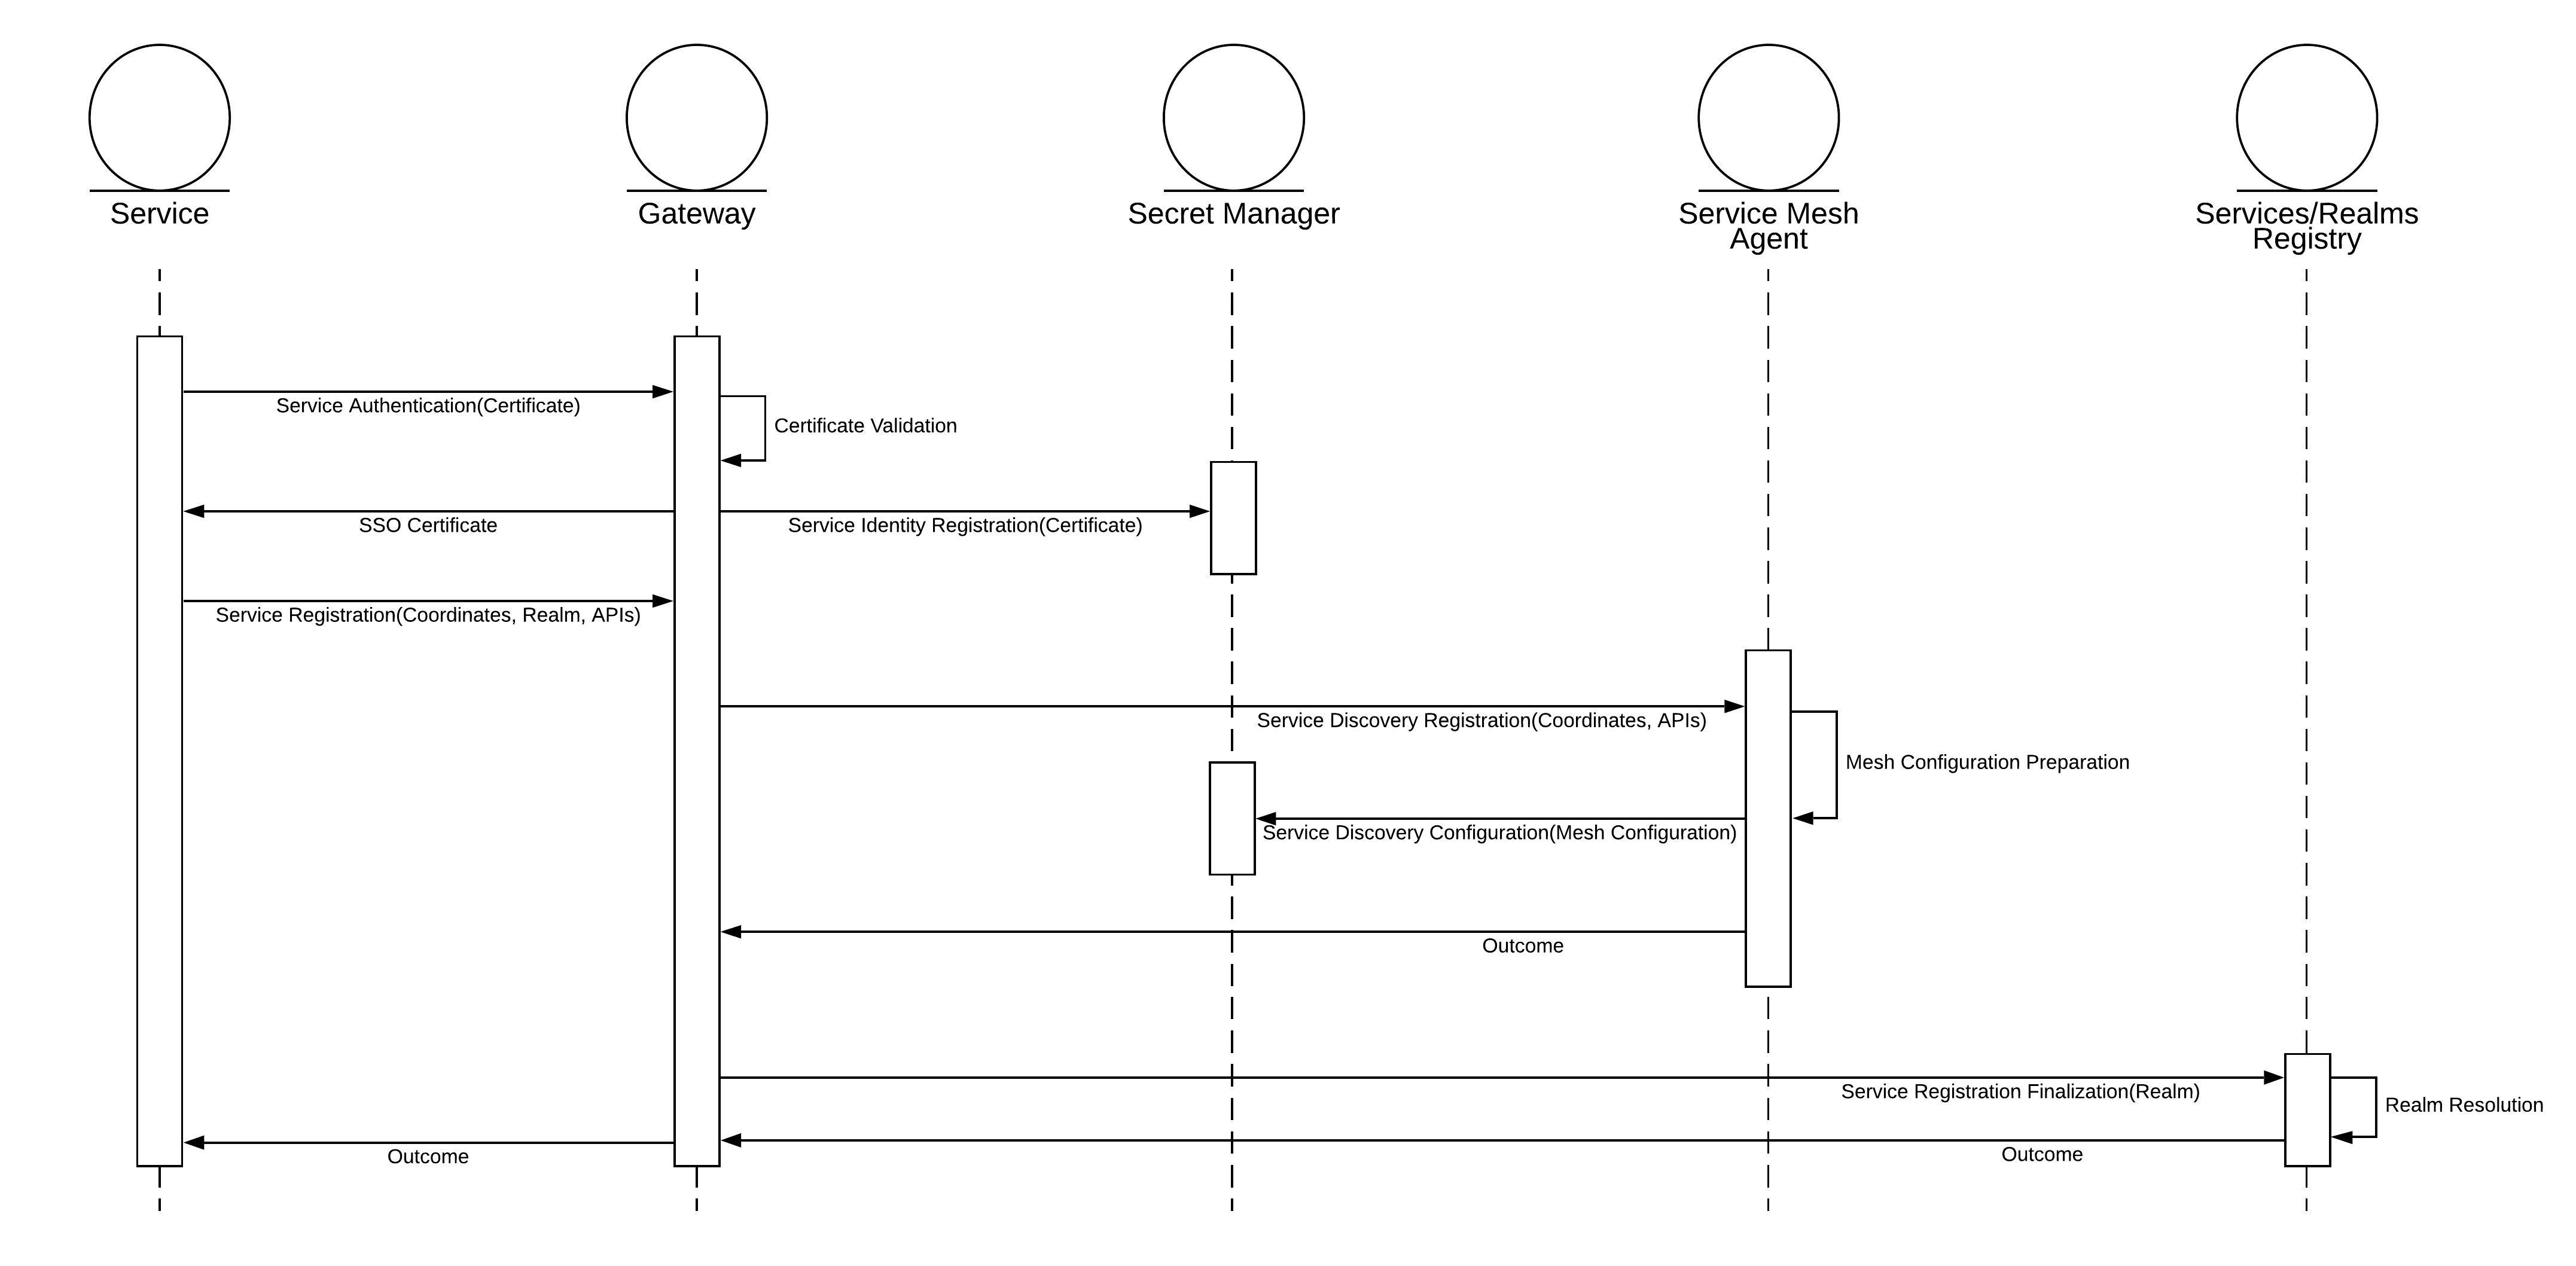
\includegraphics[scale=0.33]{Service_Registration-Sequence_Diagram.jpeg}
    \caption{Service Registration - Sequence Diagram}
    \label{fig:Service_Registration}
\end{figure}{}

\medskip
The service and SSO perform a mutual authentication by issuing each other's certificate; the SSO stores the service certificate in the vault and updates the service graph. The realm gets resolved via the Service Registry pattern.

\newpage

\subsection{User Operations}
All interactions with the Users Registry are referenced in the subsequent diagram:
\begin{figure}[h]
    \centering
    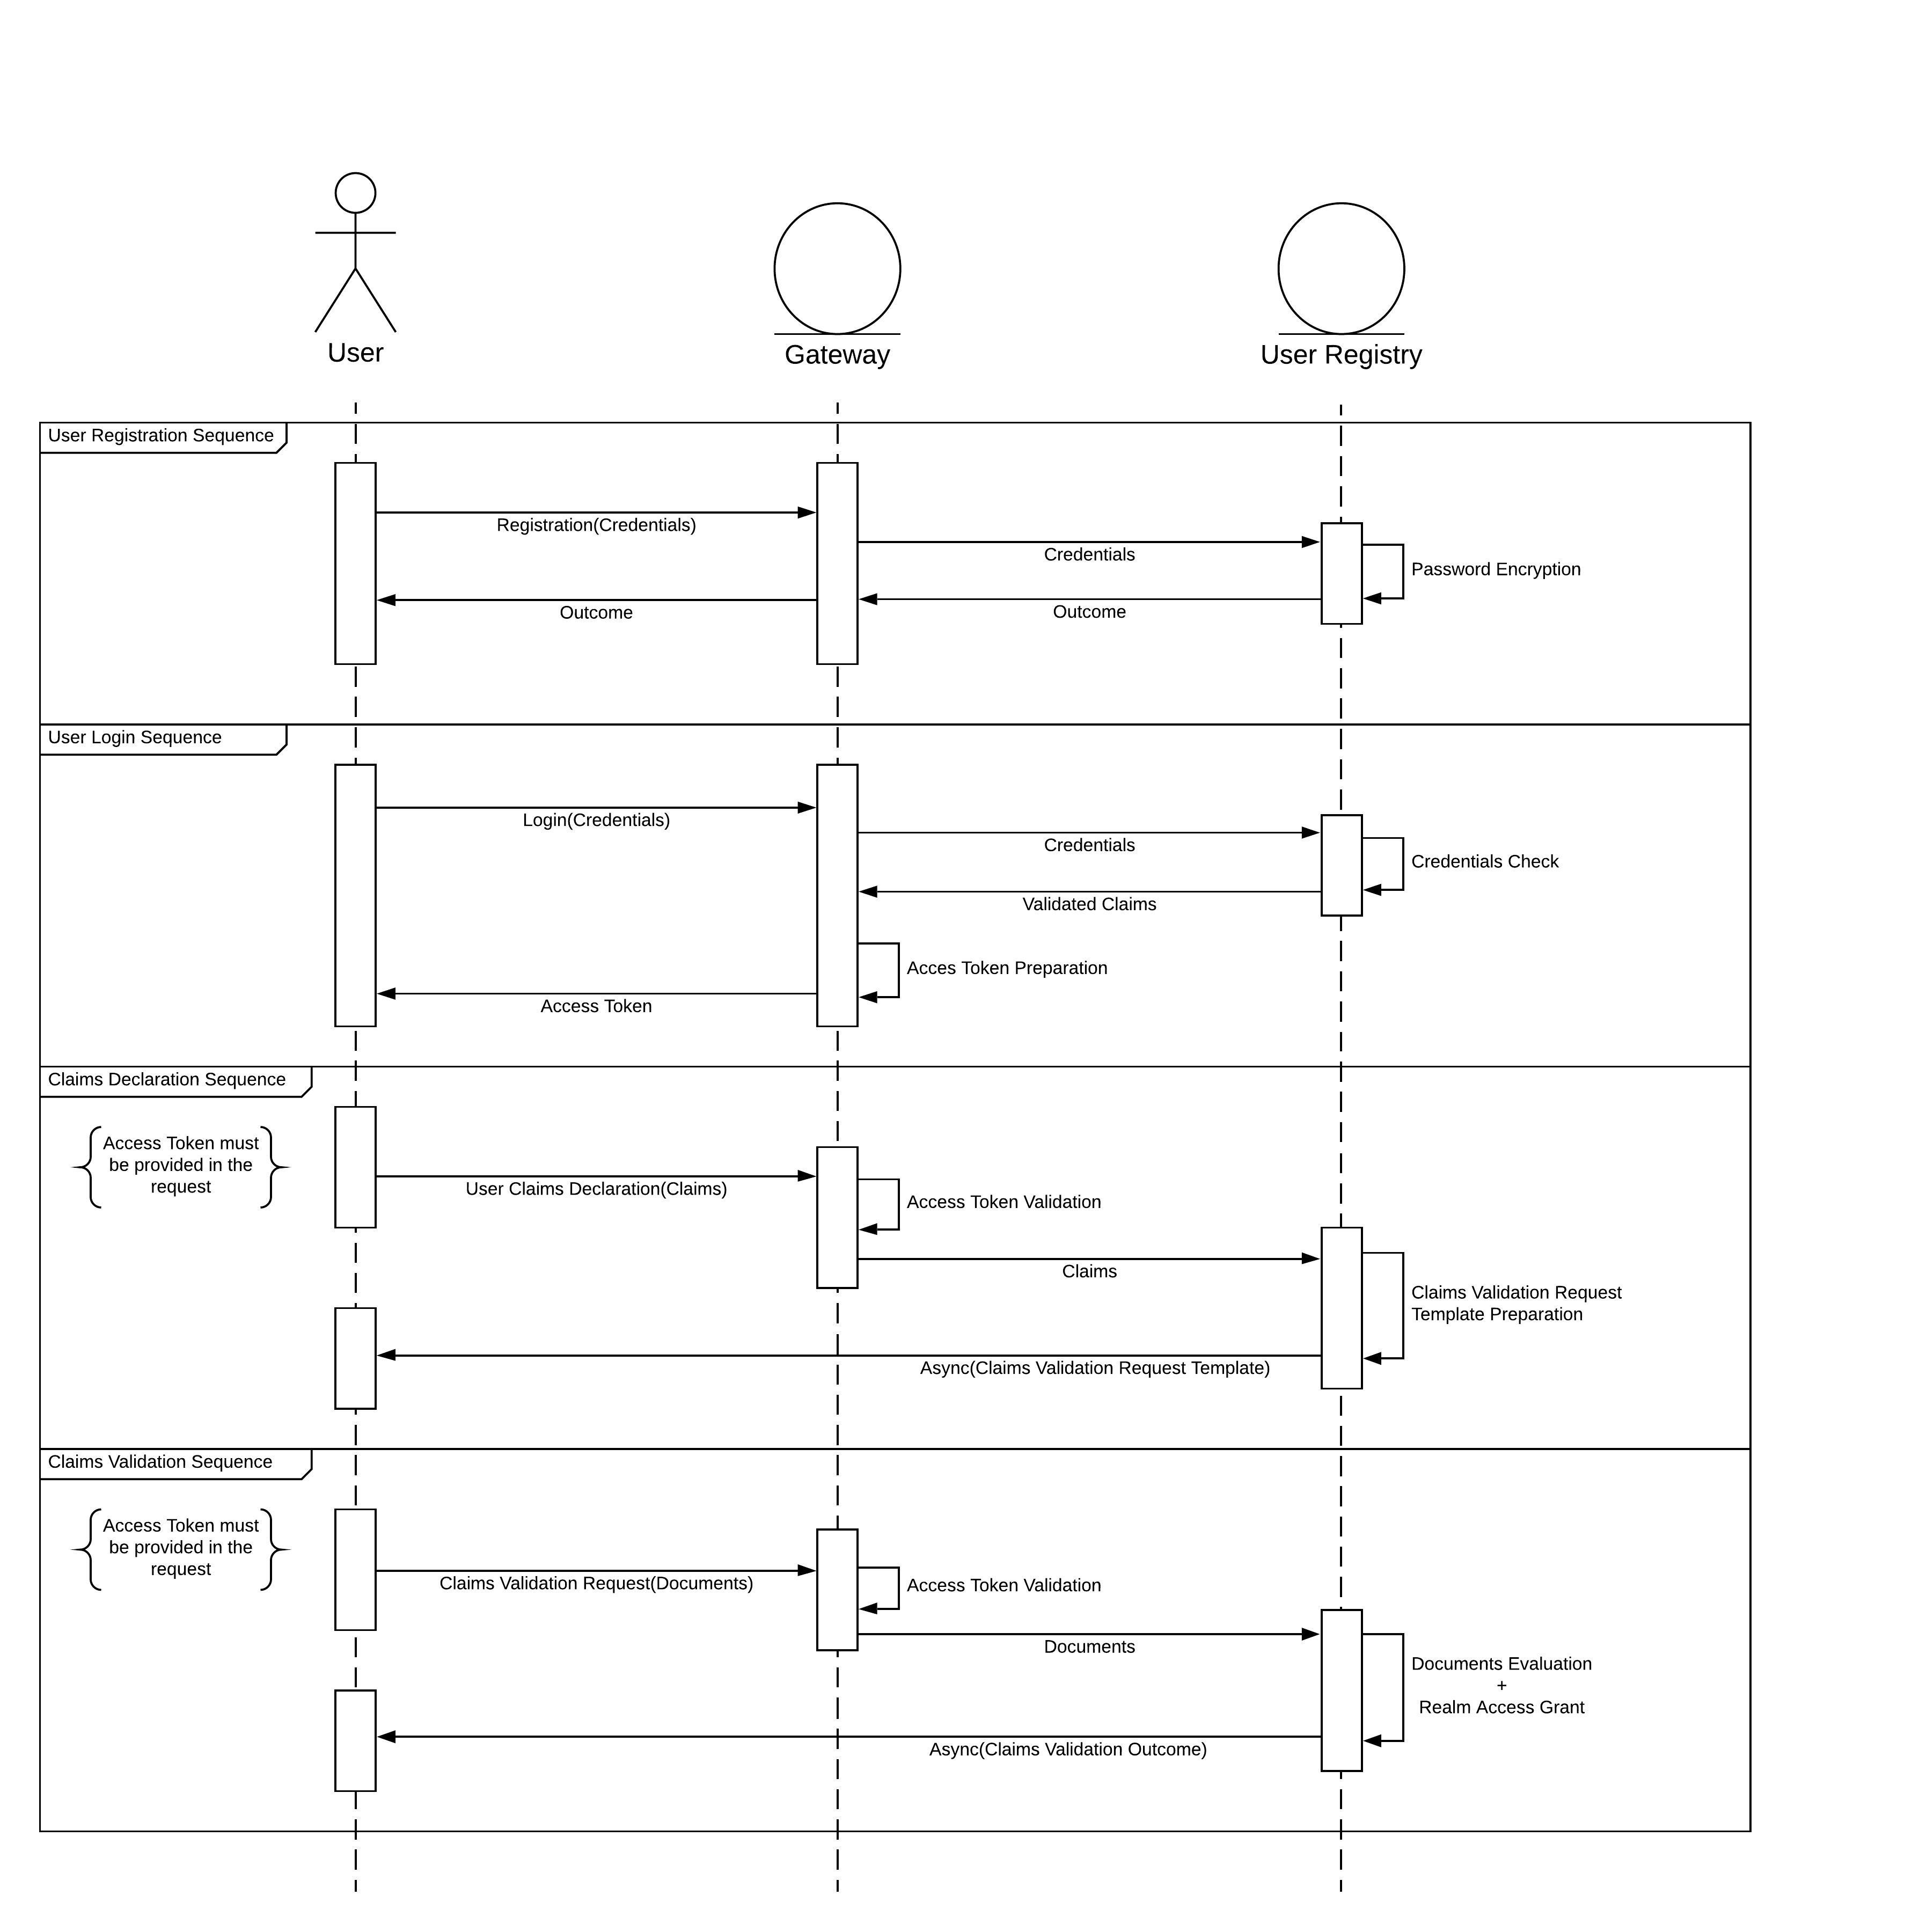
\includegraphics[scale=0.40]{Users_Operations-Sequence_Diagram.jpeg}
    \caption{User Operations - Sequence Diagram}
    \label{fig:User_Operations}
\end{figure}{}

\subsubsection{Registration}
The password is hashed via an implementation of the PBKDF2 key-derivation function described in the ``RFC-8018''\cite{PBKDF2}.\\
The function takes the password as an input and proceeds to calculate the derivation function by using 5 declared parameters:\\
\begin{itemize}
    \item Pseudo-Random Function: an efficiently computable function that emulates a \textit{random oracle}, in this case is used HMAC-SHA1;
    \item Password: the password itself;
    \item Salt: randomly generated at every function call, with a length of 64 bits as per general recommendation;
    \item Number of iterations: in this case 65536 (which produces far more entropy than common web Password-Managers use, eg. LastPass makes 5000 iterations);
    \item Key length: in this case 128.
\end{itemize}

The output of the function are the \textbf{salt} and the \textbf{hashed password}.

\subsubsection{Login}
The Access Token for users is an ``implementation''\cite{jwt.io} of the JWT (JSON Web Token) described in the ``RFC-7519''\cite{JWT}, which contains the user's identity and a representation of it's verified claims.

\subsubsection{Claims Declaration}
Registered users can independently submit their claims and will receive a Template for the  documentation needed for verify them. Each realm will have its own Template which can be extended in many sub-Templates based on the authorities that can verify the claim.

\subsubsection{Claims Validation}
For certain realms the process of claims validation can be sometimes automated: the documentation to prove the user's affinity with the realm, if defined by a "contract", can be easily evaluated. 

Some fields make use of proprietary formats which can only be judged by members of the realms, but if we take into account the possibility to register new services, third verified parties can take care of this.

\newpage

\subsection{Services Requests}
Users can interact with the registered services (if they have the necessary verified claims) via the SSO's Gateway that will take care of forwarding the request in a secured context:
\begin{figure}[h]
    \centering
    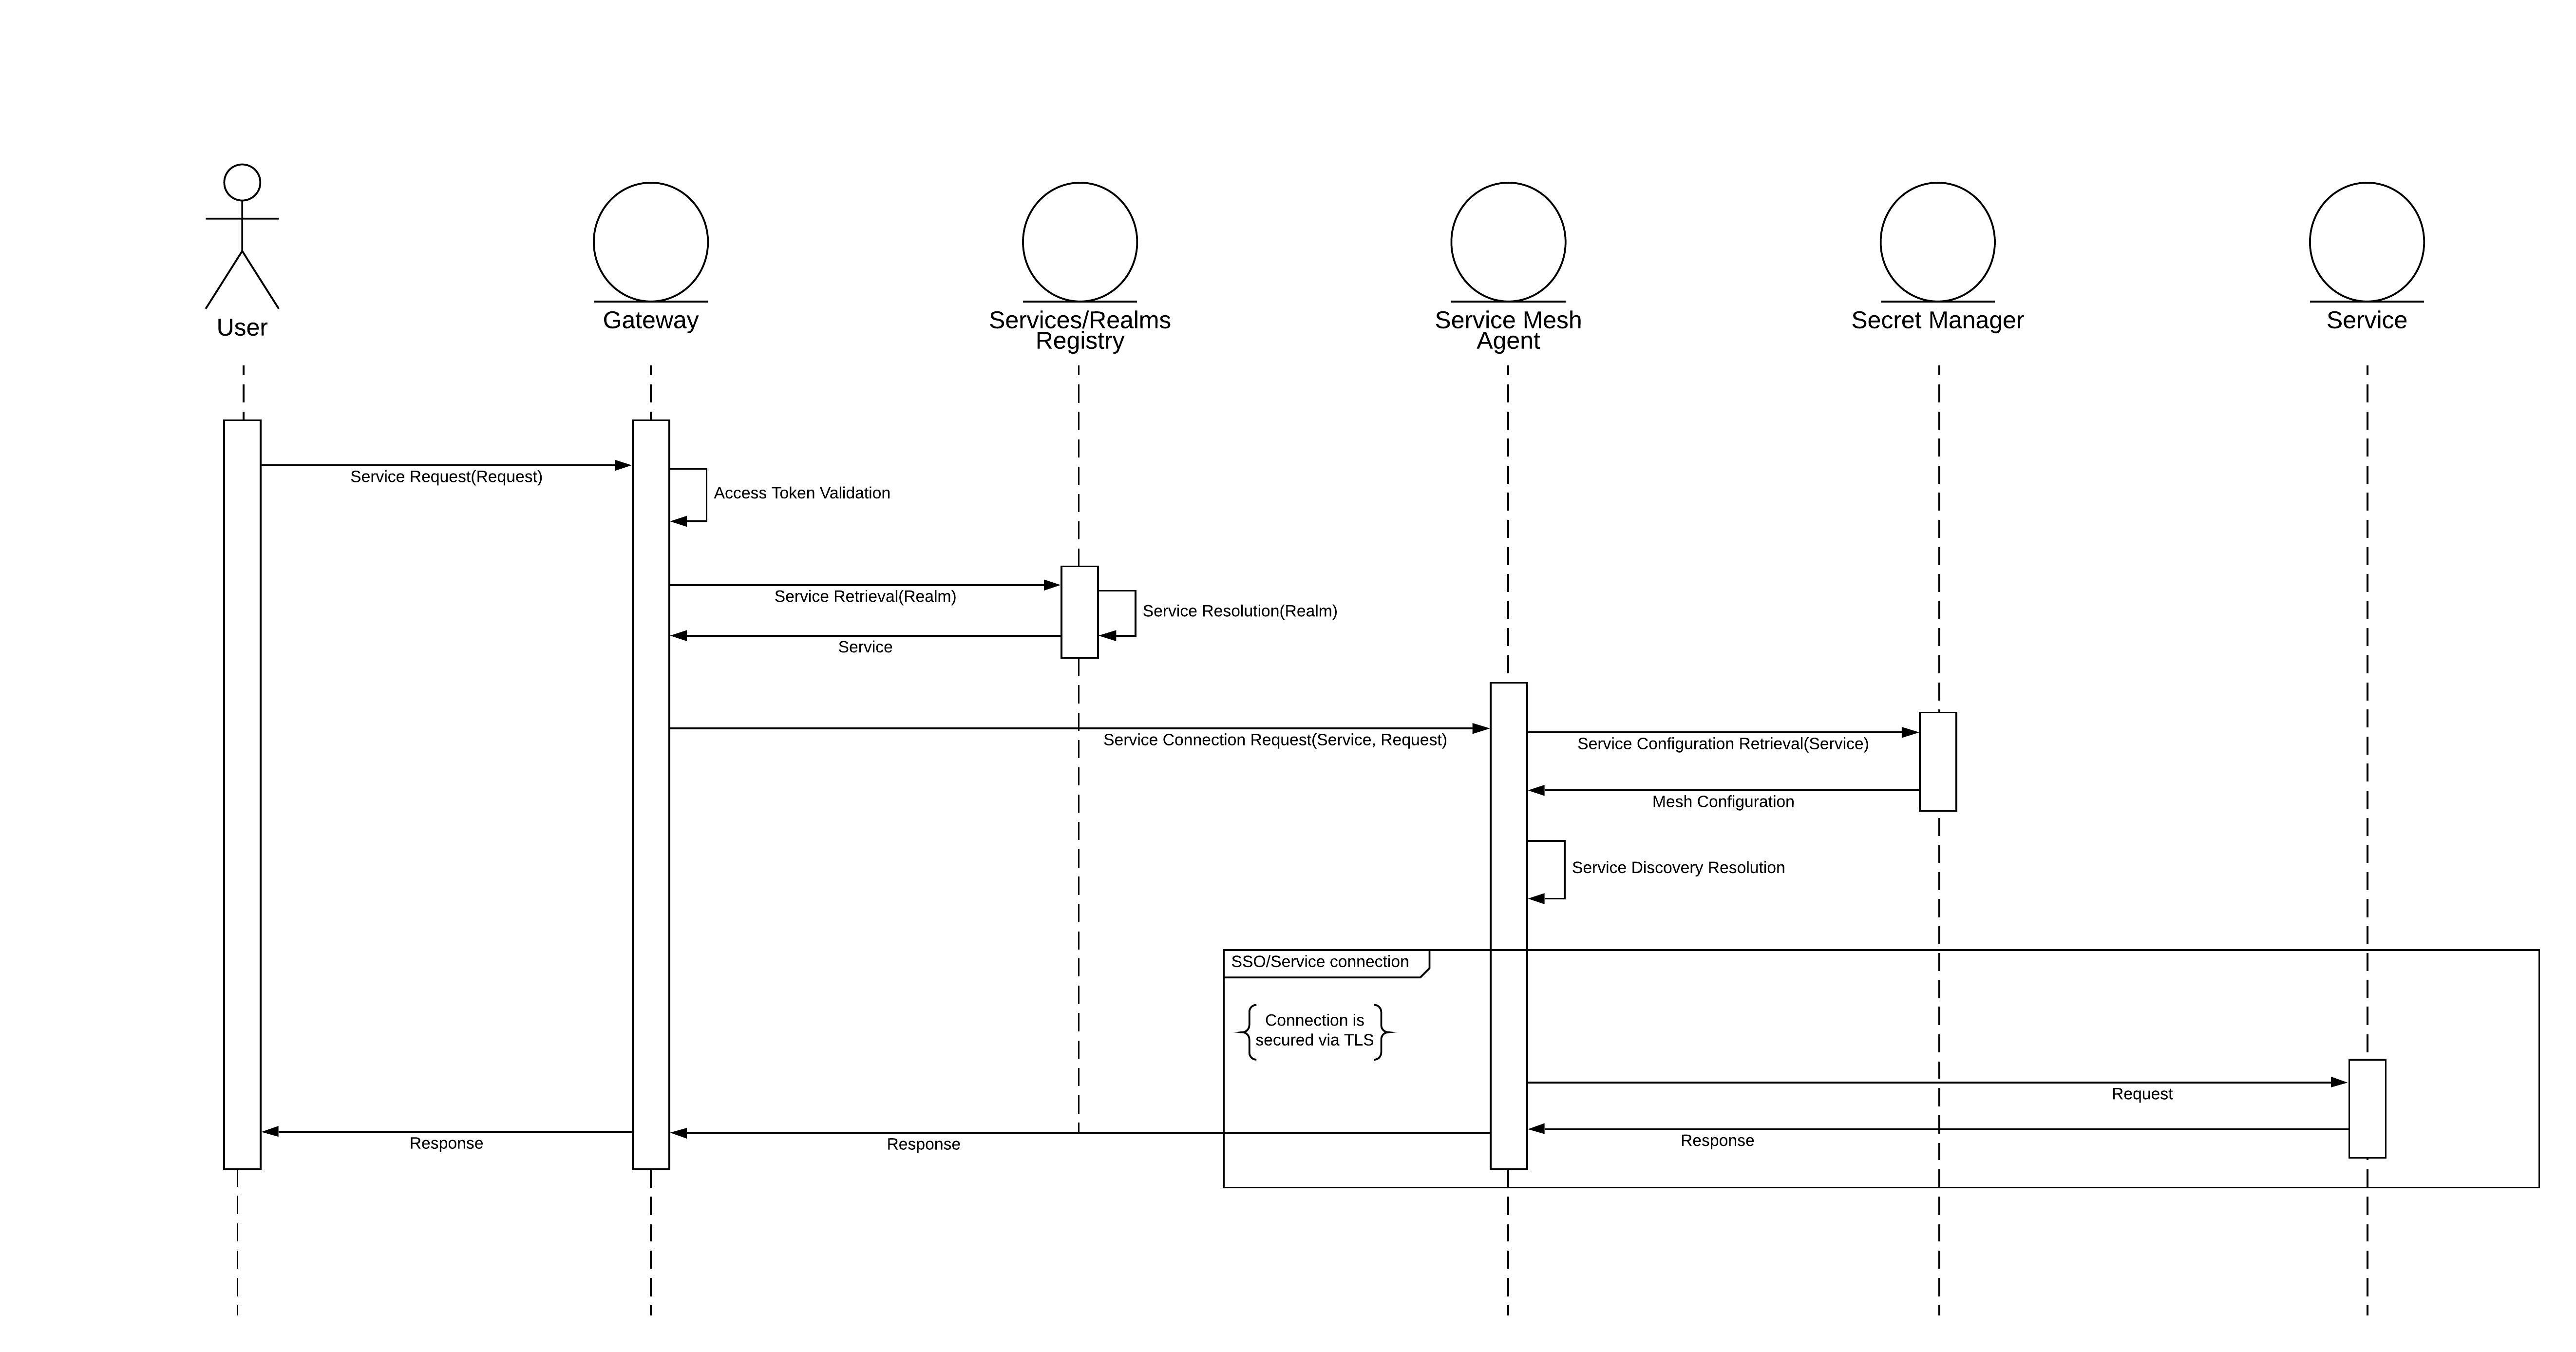
\includegraphics[scale=0.27]{Service_Request_Forwarding-Sequence_Diagram.jpeg}
    \caption{Service Request Forwarding - Sequence Diagram}
    \label{fig:Service_Request_Forwarding}
\end{figure}{}

\newpage

\section{Conclusions}
The main difference between the solution and a traditional SSO like ``Kerberos''\cite{kerberos} is about granting \textbf{service availability and connection responsibility} as core features.\\
Kerberos provides the User with the ticket needed to authenticate with a service, but the subsequent interactions with it are entirely delegated to the user.
\medskip

In the presented SSO solution the responsibility is not delegated and takes care of the security of the communication channel with the service forwarding the user's request.\\
In a distributed environment, if the registered services have interactions within their contexts besides the SSO flow-control and implement the Service Mesh Agent, the SSO can still be aware of what is going on.\\
The service graph will always be updated and the health-check monitor will catch eventual failures, circuit-breaking the requests and securing the users from attacks.

\newpage

\bibliographystyle{unsrt}
\bibliography{references}
\end{document}
